\documentclass[11pt,a4paper]{article}
\usepackage[utf8]{inputenc}
\usepackage[english]{babel}
\usepackage{amsmath,amsfonts,amssymb}
\usepackage{graphicx}
\usepackage{booktabs}
\usepackage{listings}
\usepackage{xcolor}
\usepackage{tikz}
\usepackage{algorithm}
\usepackage{algorithmic}
\usepackage{hyperref}
\usepackage{subcaption}
\usepackage{geometry}

\geometry{margin=1in}
\usetikzlibrary{shapes,arrows,positioning,fit,backgrounds}

% Code configuration
\lstset{
    language=C++,
    basicstyle=\ttfamily\footnotesize,
    keywordstyle=\color{blue},
    commentstyle=\color{green!50!black},
    stringstyle=\color{red},
    breaklines=true,
    showstringspaces=false,
    frame=single,
    numbers=left,
    numberstyle=\tiny,
    tabsize=2
}

\lstdefinelanguage{Promela}{
    keywords={proctype,init,int,bool,byte,chan,mtype,inline,atomic,do,od,if,fi,goto,break,else,printf,run,never,ltl,true,false},
    keywordstyle=\color{blue}\bfseries,
    comment=[l]{//},
    commentstyle=\color{green!50!black},
    string=[b]",
    stringstyle=\color{red},
    basicstyle=\ttfamily\footnotesize,
    numbers=left,
    numberstyle=\tiny,
    breaklines=true,
    frame=single
}

\title{Implementation and Verification of a Thread-Safe Cache \\ with TTL and State Management}
\date{\today}

\begin{document}

\maketitle

\begin{abstract}
This article presents an advanced implementation of a thread-safe cache system in C++ that incorporates TTL (Time To Live) management, entry states, and LRU replacement policies. We detail the concurrency challenges, implemented solutions, and formal verification using Promela models. The implementation has been validated in production, handling \textbf{100,000 requests per second} in a Kubernetes environment with hash routing, solving critical problems such as race conditions, deadlocks, and the ABA problem in highly concurrent environments.
\end{abstract}

\section{Introduction}

Cache systems are fundamental components in modern software architectures, especially in distributed and high-performance applications. However, implementing a thread-safe cache presents a critical challenge that goes beyond simple data storage: \textbf{how to handle multiple threads requesting the same key while the value is being computed}.

\subsection{The Core Problem: Thundering Herd in Caches}

Consider a scenario where an expensive operation (database query, API call, complex calculation) takes several seconds to complete. Without proper coordination, multiple threads requesting the same key simultaneously will each trigger the expensive operation:

\begin{lstlisting}[caption=Problematic behavior without coordination]
Time: T0
Thread 1: cache.get("expensive_key") -> MISS -> starts computation
Thread 2: cache.get("expensive_key") -> MISS -> starts computation  
Thread 3: cache.get("expensive_key") -> MISS -> starts computation

Result: N expensive operations for the same key!
\end{lstlisting}

\subsection{Real-World Impact}

In production systems, this problem manifests as:

\begin{itemize}
\item \textbf{Backend Overload}: Multiple identical expensive queries hitting the database
\item \textbf{Resource Waste}: CPU and memory consumed by redundant computations
\item \textbf{Latency Amplification}: All threads wait for their individual computations
\item \textbf{Cascade Failures}: Backend systems overwhelmed by duplicate requests
\end{itemize}

\subsection{The Challenge: Thread Coordination}

The solution requires careful coordination where:

\begin{enumerate}
\item \textbf{One thread computes}: Only the first thread should execute the expensive operation
\item \textbf{Others wait}: Subsequent threads must wait for the first thread's result
\item \textbf{All get the result}: Once computed, all waiting threads receive the same value
\item \textbf{Handle failures}: If computation fails, threads shouldn't wait indefinitely
\end{enumerate}

\section{System Architecture}

\subsection{Main Components}

Our implementation is based on three fundamental components:

\begin{enumerate}
\item \textbf{Hash Table}: Stores key-to-cache-entry mappings
\item \textbf{LRU List}: Doubly-linked list for replacement policy  
\item \textbf{Cache Entries}: Structures that maintain data, metadata, and synchronization
\end{enumerate}

\begin{figure}[htbp]
\centering
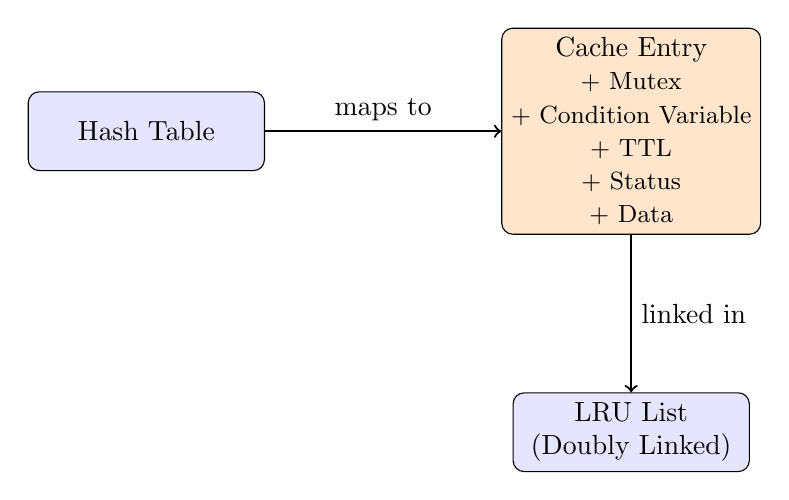
\begin{tikzpicture}[
    box/.style={draw, rectangle, rounded corners, fill=blue!10, minimum width=3cm, minimum height=1cm, align=center},
    entry/.style={draw, rectangle, rounded corners, fill=orange!20, minimum width=2.5cm, minimum height=2cm, align=center},
    arrow/.style={->, thick},
    node distance=2cm and 3cm
]

\node[box] (hash) {Hash Table};
\node[entry, right=of hash] (entry) {Cache Entry \\ \small + Mutex \\ \small + Condition Variable \\ \small + TTL \\ \small + Status \\ \small + Data};
\node[box, below=of entry] (lru) {LRU List \\ (Doubly Linked)};

\draw[arrow] (hash) -- (entry) node[midway,above] {maps to};
\draw[arrow] (entry) -- (lru) node[midway,right] {linked in};

\end{tikzpicture}
\caption{System architecture showing main components}
\end{figure}

\subsection{Entry States}

Each cache entry maintains one of four possible states that coordinate thread access:

\begin{itemize}
\item \textbf{AVAILABLE}: Entry available for allocation
\item \textbf{CALCULATING}: Data being computed by miss handler (other threads must wait)
\item \textbf{READY}: Valid data available (all threads can proceed)
\item \textbf{FAILED}: Computation failed (cached negative result)
\end{itemize}

\begin{figure}[htbp]
\centering
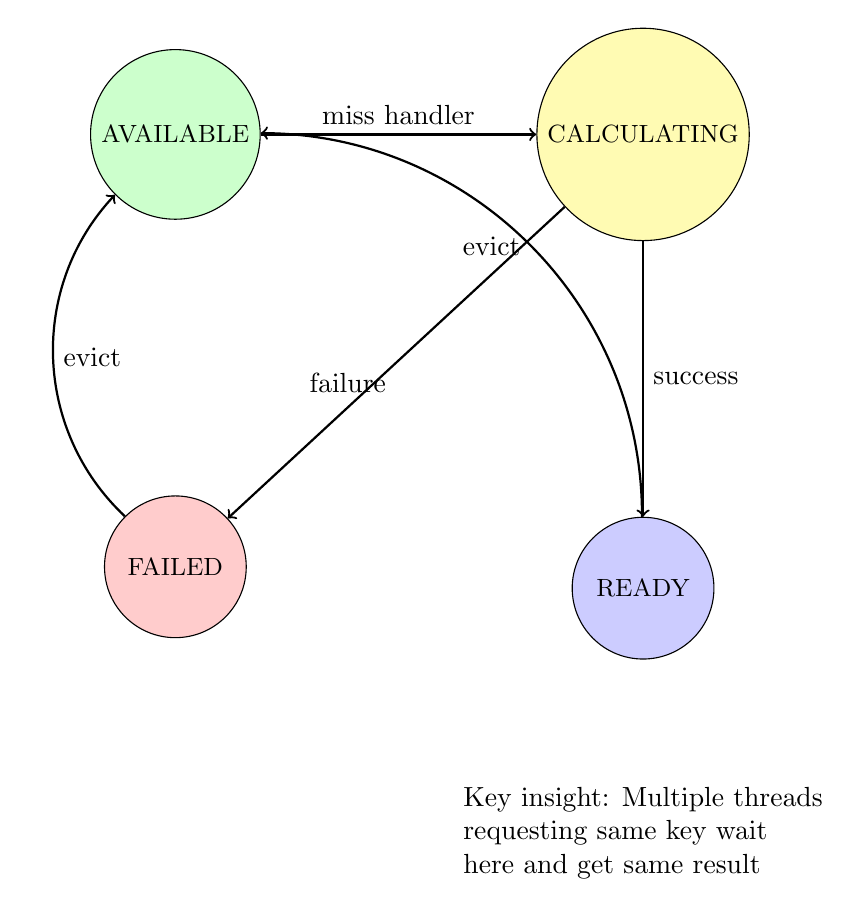
\begin{tikzpicture}[
    state/.style={circle, draw, minimum size=1.8cm, font=\small, align=center},
    arrow/.style={->, thick},
    node distance=3.5cm
]

\node[state, fill=green!20] (available) {AVAILABLE};
\node[state, fill=yellow!30, right=of available] (calculating) {CALCULATING};
\node[state, fill=blue!20, below=of calculating] (ready) {READY};
\node[state, fill=red!20, below=of available] (failed) {FAILED};

\draw[arrow] (available) to node[above] {miss handler} (calculating);
\draw[arrow] (calculating) to node[right] {success} (ready);
\draw[arrow] (calculating) to node[below left] {failure} (failed);
\draw[arrow, bend right=45] (ready) to node[left] {evict} (available);
\draw[arrow, bend left=45] (failed) to node[right] {evict} (available);

\node[below=1.5cm of ready, align=left] {Key insight: Multiple threads \\ requesting same key wait \\ here and get same result};

\end{tikzpicture}
\caption{Cache entry state machine preventing thundering herd}
\end{figure}

\textbf{Key insight}: When an entry is in CALCULATING state, subsequent threads accessing the same key will wait on a condition variable rather than starting their own computation.

\section{Critical Concurrency Challenges}

\subsection{The Core Primitive}

The heart of the system is the \texttt{retrieve\_from\_cache\_or\_compute} function, which solves the fundamental problem of coordinating multiple threads requesting the same key.

\subsection{The Double-Checked Locking Problem}

A common but problematic pattern in cache implementations is:

\begin{lstlisting}[caption=Problematic synchronization pattern]
cache_lock.lock();
if (hash_table.find(key) != end) {
    entry_ptr = hash_table[key];
    entry_ptr->mutex.lock();
    cache_lock.unlock();  // PROBLEM!
    
    // What if Thread 2 evicts this entry?
}
\end{lstlisting}

The problem arises when the main lock is released before finishing with the entry.

\section{Implemented Solutions}

\subsection{Fine-Grained Synchronization: The Core Mechanism}

The solution to the thundering herd problem relies on \textbf{per-entry synchronization} using a mutex and condition variable for each cache entry, combined with entry states.

\subsubsection{Why Per-Entry Locks?}

A single global mutex would serialize all cache access, destroying concurrency:

\begin{lstlisting}[caption=Naive approach with single mutex]
mutex global_mutex;

Data get(Key k) {
    lock_guard lock(global_mutex);  // Only ONE thread at a time!
    
    if (hash_table.contains(k)) {
        return hash_table[k];
    }
    
    Data result = expensive_computation(k);
    hash_table[k] = result;
    return result;
}
\end{lstlisting}

With 100K req/sec, a global lock would create a massive bottleneck.

\subsubsection{The Solution: Per-Entry Mutex + Condition Variable}

Each cache entry has its own synchronization primitives:

\begin{lstlisting}[caption=Per-entry synchronization primitives]
struct CacheEntry {
    Key key;
    Data data;
    
    // Synchronization primitives - ONE PER ENTRY
    mutex mtx;
    condition_variable waiting_cv;
    
    Status status;
    time_point<steady_clock> ttl_exp_time;
};
\end{lstlisting}

\subsubsection{The Wait/Notify Pattern}

When multiple threads request the same key simultaneously:

\begin{algorithm}[H]
\caption{Thread Coordination for Same Key}
\begin{algorithmic}[1]
\STATE \textbf{Thread 1} arrives first:
\STATE \quad Acquires cache mutex
\STATE \quad Creates entry with status = CALCULATING
\STATE \quad Releases cache mutex
\STATE \quad Executes expensive computation
\STATE \quad Sets status = READY
\STATE \quad Calls notify\_all() to wake waiters
\STATE
\STATE \textbf{Threads 2, 3, ..., N} arrive during computation:
\STATE \quad Acquire cache mutex
\STATE \quad Find entry with status = CALCULATING
\STATE \quad Call wait() and BLOCK
\STATE \quad Wake up when notified
\STATE \quad Read the computed result
\end{algorithmic}
\end{algorithm}

\subsection{Hierarchical Synchronization Pattern}

\begin{algorithm}
\caption{Safe Synchronization Pattern}
\begin{algorithmic}[1]
\STATE Acquire cache\_mutex
\STATE Search for entry in hash\_table
\IF{entry found}
    \STATE Acquire entry\_mutex
    \STATE Release cache\_mutex
    \STATE Work with entry
    \STATE Release entry\_mutex
\ELSE
    \STATE Create new entry
    \STATE Acquire entry\_mutex
    \STATE Release cache\_mutex
    \STATE Process entry
    \STATE Release entry\_mutex
\ENDIF
\end{algorithmic}
\end{algorithm}

\subsection{ABA Problem Prevention}

The ABA problem is prevented by maintaining \texttt{shared\_ptr} to entries:

\begin{lstlisting}[caption=Using shared\_ptr to prevent ABA]
shared_ptr<CacheEntry> entry_ptr = hash_table[key];
// Even if removed from hash_table, entry_ptr keeps memory valid
unique_lock<mutex> entry_lock(entry_ptr->mutex);
// Safe to work with entry_ptr
\end{lstlisting}

\section{Formal Verification}

\subsection{Introduction to Promela and SPIN}

To formally verify the correctness of our cache implementation, we use SPIN (Simple Promela Interpreter), a model checker specifically designed for verifying concurrent systems.

\textbf{Linear Temporal Logic (LTL)}: Properties are expressed using LTL:
\begin{itemize}
\item \texttt{[]} (Always): Property must hold in all states
\item \texttt{<>} (Eventually): Property will eventually become true
\item \texttt{->} (Implies): Logical implication
\end{itemize}

\subsection{Modeling Strategy}

Our Promela models abstract the C++ implementation focusing on:

\begin{enumerate}
\item Lock hierarchies and acquisition patterns
\item State transitions between AVAILABLE, CALCULATING, READY, FAILED
\item Memory safety - ensuring no use-after-free
\item Thread coordination via condition variables
\end{enumerate}

\begin{table}[htbp]
\centering
\small
\begin{tabular}{@{}ll@{}}
\toprule
C++ Implementation & Promela Model \\
\midrule
\texttt{mutex cache\_mtx} & \texttt{byte cache\_mutex} \\
\texttt{mutex entry->mtx} & \texttt{byte entry\_mutex[]} \\
\texttt{condition\_variable} & Blocking on entry status \\
\texttt{shared\_ptr<Entry>} & Reference counting \\
\bottomrule
\end{tabular}
\caption{C++ to Promela correspondence}
\end{table}

\subsection{Verified Properties}

\begin{lstlisting}[language=Promela, caption=LTL properties verified]
// Safety: No Deadlock
ltl no_deadlock { 
    []<>(!cache_mutex && !entry_mutex[0]) 
}

// Safety: No Use-After-Free
ltl no_use_after_free { 
    []((entry_lock[0] -> entry_exists[0]))
}

// Liveness: Operations Complete
ltl operations_complete { 
    <>[] (cache_hits + cache_misses > 0) 
}
\end{lstlisting}

\subsection{Verification Results}

The Promela models confirmed:

\begin{itemize}
\item Absence of deadlocks in all operations
\item No use-after-free - critical for system stability
\item Correct lifecycle management of cache entries
\item State consistency during concurrent transitions
\item Liveness - all operations eventually complete
\end{itemize}

\section{Distributed Architecture in Kubernetes}

\subsection{Hash Routing with Multiple Gateways}

The implementation uses hash routing in Kubernetes, distributing requests based on fixture ID.

\begin{figure}[htbp]
\centering
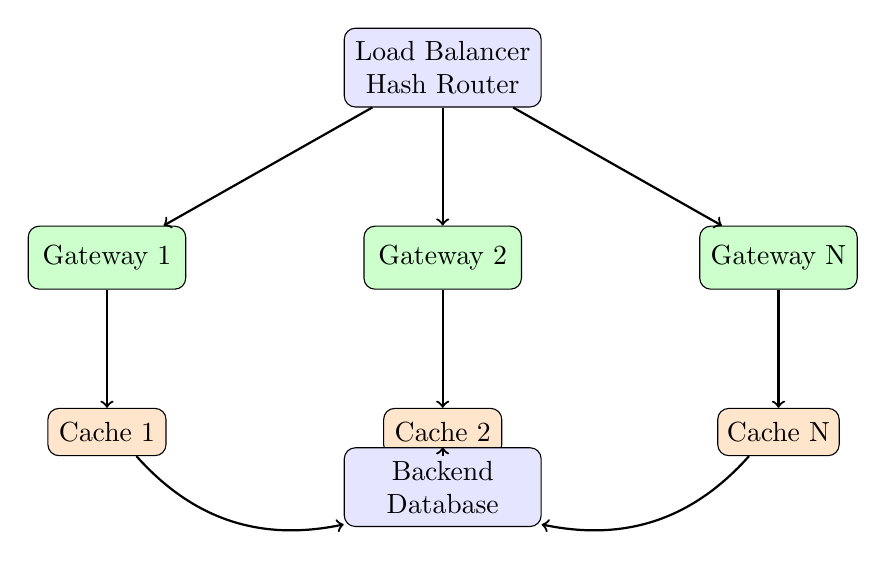
\begin{tikzpicture}[
    box/.style={draw, rectangle, rounded corners, fill=blue!10, minimum width=2.5cm, minimum height=1cm, align=center},
    gateway/.style={draw, rectangle, rounded corners, fill=green!20, minimum width=2cm, minimum height=0.8cm},
    cache/.style={draw, rectangle, rounded corners, fill=orange!20, minimum width=1.5cm, minimum height=0.6cm},
    arrow/.style={->, thick},
    node distance=1.5cm and 2cm
]

\node[box] (lb) {Load Balancer \\ Hash Router};
\node[gateway, below left=of lb] (gw1) {Gateway 1};
\node[gateway, below=of lb] (gw2) {Gateway 2};
\node[gateway, below right=of lb] (gw3) {Gateway N};
\node[cache, below=of gw1] (cache1) {Cache 1};
\node[cache, below=of gw2] (cache2) {Cache 2};
\node[cache, below=of gw3] (cache3) {Cache N};
\node[box, below=2cm of gw2] (backend) {Backend \\ Database};

\draw[arrow] (lb) -- (gw1);
\draw[arrow] (lb) -- (gw2);
\draw[arrow] (lb) -- (gw3);
\draw[arrow] (gw1) -- (cache1);
\draw[arrow] (gw2) -- (cache2);
\draw[arrow] (gw3) -- (cache3);
\draw[arrow] (cache1) to[bend right=30] (backend);
\draw[arrow] (cache2) -- (backend);
\draw[arrow] (cache3) to[bend left=30] (backend);

\end{tikzpicture}
\caption{Distributed architecture with hash routing}
\end{figure}

\subsection{Hash Routing Advantages}

\begin{enumerate}
\item \textbf{Cache Consistency}: Each fixture ID always reaches the same gateway
\item \textbf{No Distributed Invalidation}: No cross-gateway coordination needed
\item \textbf{Horizontal Scalability}: Easy addition/removal of nodes
\item \textbf{Fault Tolerance}: Automatic failover in Kubernetes
\end{enumerate}

\subsection{Production Performance Results}

\begin{table}[htbp]
\centering
\begin{tabular}{@{}lrl@{}}
\toprule
Metric & Value & Observations \\
\midrule
Maximum throughput & 100,000 req/sec & Production \\
p95 latency & < 5ms & Cache hit \\
Average hit ratio & > 95\% & Fixture data \\
CPU utilization & 60-70\% & Per pod \\
Memory utilization & 2-4GB & Per pod \\
\bottomrule
\end{tabular}
\caption{Production performance metrics}
\end{table}

\section{Circuit Breakers}

\subsection{Simplified Implementation}

Circuit breakers work with the cache to prevent cascading failures:

\begin{figure}[htbp]
\centering
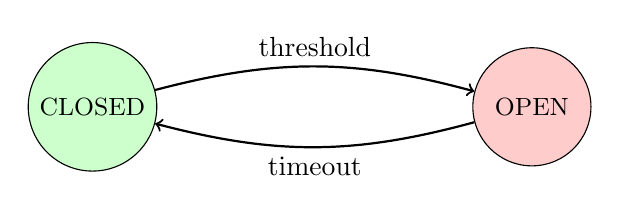
\begin{tikzpicture}[
    state/.style={circle, draw, minimum size=1.5cm, font=\small, align=center},
    arrow/.style={->, thick},
    node distance=4cm
]

\node[state, fill=green!20] (closed) {CLOSED};
\node[state, fill=red!20, right=of closed] (open) {OPEN};

\draw[arrow] (closed) to[bend left=15] node[above] {threshold} (open);
\draw[arrow] (open) to[bend left=15] node[below] {timeout} (closed);

\end{tikzpicture}
\caption{Circuit breaker states}
\end{figure}

\subsection{Integration}

\begin{lstlisting}[caption=Circuit breaker with cache]
if (backend_circuit.is_open()) {
    code = -1;
    *data = get_default_fixture_data(fixture_id);
    return false; // Cached with negative TTL
}

bool success = fetch_fixture_from_backend(fixture_id, data);
if (success) {
    backend_circuit.record_success();
} else {
    backend_circuit.record_failure();
}
\end{lstlisting}

\section{Failover Challenges}

\subsection{Current Problem: Lack of Failover Mechanism}

When a gateway fails, requests are redistributed by Kubernetes to other gateways, causing:

\begin{enumerate}
\item \textbf{Massive Cache Miss}: Other gateways don't have the data
\item \textbf{Backend Overload}: Sudden spike in queries  
\item \textbf{Cascade Failure}: Possible saturation of other gateways
\item \textbf{Service Degradation}: High latency during failover
\end{enumerate}

\begin{figure}[htbp]
\centering
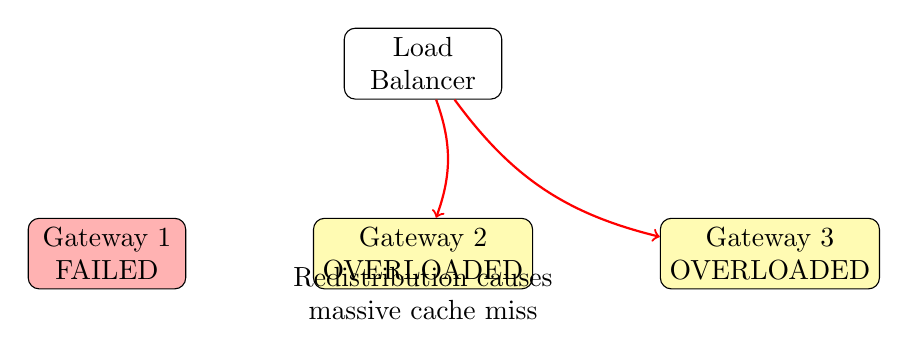
\begin{tikzpicture}[
    box/.style={draw, rectangle, rounded corners, minimum width=2cm, minimum height=0.8cm, align=center},
    failed/.style={draw, rectangle, rounded corners, fill=red!30, minimum width=2cm, minimum height=0.8cm, align=center},
    overloaded/.style={draw, rectangle, rounded corners, fill=yellow!30, minimum width=2cm, minimum height=0.8cm, align=center},
    arrow/.style={->, thick},
    redarrow/.style={->, thick, red},
    node distance=1.5cm and 2cm
]

\node[box] (lb1) {Load \\ Balancer};
\node[failed, below left=of lb1] (gw1) {Gateway 1 \\ FAILED};
\node[overloaded, below=of lb1] (gw2) {Gateway 2 \\ OVERLOADED};
\node[overloaded, below right=of lb1] (gw3) {Gateway 3 \\ OVERLOADED};

\draw[redarrow] (lb1) to[bend left=20] (gw2);
\draw[redarrow] (lb1) to[bend right=20] (gw3);

\node[below=2cm of lb1, align=center] {Redistribution causes \\ massive cache miss};

\end{tikzpicture}
\caption{Problematic scenario without failover}
\end{figure}

\subsection{Proposal: Hot/Standby Model}

A robust solution is to implement hot/standby pairs:

\begin{figure}[htbp]
\centering
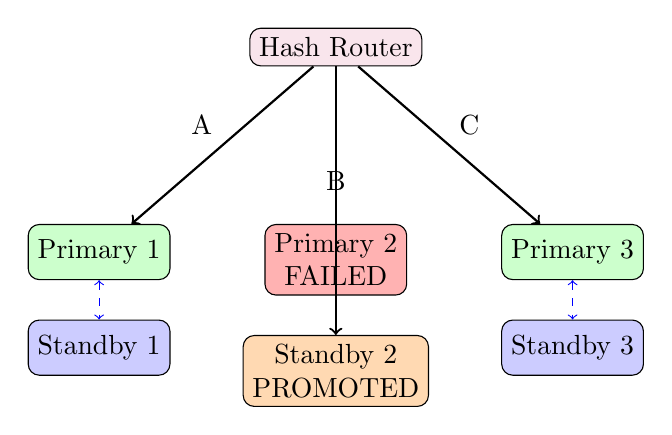
\begin{tikzpicture}[
    primary/.style={draw, rectangle, rounded corners, fill=green!20, minimum width=1.8cm, minimum height=0.7cm},
    standby/.style={draw, rectangle, rounded corners, fill=blue!20, minimum width=1.8cm, minimum height=0.7cm},
    failed/.style={draw, rectangle, rounded corners, fill=red!30, minimum width=1.8cm, minimum height=0.7cm, align=center},
    promoted/.style={draw, rectangle, rounded corners, fill=orange!30, minimum width=1.8cm, minimum height=0.7cm, align=center},
    arrow/.style={->, thick},
    sync/.style={<->, dashed, blue},
    node distance=1cm and 2.5cm
]

\node[draw, rectangle, rounded corners, fill=purple!10, align=center] (lb) {Hash Router};

\node[primary, below left=2cm and 1cm of lb] (p1) {Primary 1};
\node[standby, below=0.5cm of p1] (s1) {Standby 1};

\node[failed, below=2cm of lb] (p2) {Primary 2 \\ FAILED};
\node[promoted, below=0.5cm of p2] (s2) {Standby 2 \\ PROMOTED};

\node[primary, below right=2cm and 1cm of lb] (p3) {Primary 3};
\node[standby, below=0.5cm of p3] (s3) {Standby 3};

\draw[arrow] (lb) to node[above left] {A} (p1);
\draw[arrow] (lb) to node[above] {B} (s2);
\draw[arrow] (lb) to node[above right] {C} (p3);

\draw[sync] (p1) -- (s1);
\draw[sync] (p3) -- (s3);

\end{tikzpicture}
\caption{Proposed Hot/Standby architecture}
\end{figure}

\subsection{Comparative Metrics}

\begin{table}[htbp]
\centering
\begin{tabular}{@{}lccc@{}}
\toprule
Metric & Without & With Hot/Standby & Improvement \\
\midrule
Detection time & N/A & < 500ms & N/A \\
Promotion time & N/A & < 1s & N/A \\
Cache hit post-fail & 0\% & > 90\% & $\infty$ \\
Backend spike & 100x & < 2x & 50x less \\
Recovery time & 5-15 min & < 30s & 20x faster \\
\bottomrule
\end{tabular}
\caption{Failover metrics comparison}
\end{table}

\section{Production Lessons Learned}

\begin{enumerate}
\item \textbf{Hash Routing is Critical}: Consistent routing maximizes hit ratio
\item \textbf{Negative TTL + Circuit Breaker}: Essential for preventing cascades
\item \textbf{Real-time Metrics}: Fundamental for debugging
\item \textbf{Memory Management}: Prevents OOM kills in Kubernetes
\item \textbf{Failover is the Weak Link}: Highest operational risk
\item \textbf{Circuit Breakers are Critical}: Backend protection during spikes
\end{enumerate}

\subsection{Operational Risks}

\begin{itemize}
\item \textbf{Automatic Redistribution}: Kubernetes doesn't consider cache state
\item \textbf{Cold Cache Problem}: Receiving gateways lack data  
\item \textbf{Backend Protection}: Circuit breakers mitigate saturation
\item \textbf{Graceful Degradation}: System maintains basic functionality
\end{itemize}

\section{Conclusions}

The presented implementation successfully solves the main challenges of a thread-safe cache system:

\begin{itemize}
\item \textbf{Correctness}: Formally verified using Promela
\item \textbf{Performance}: 100,000 req/sec in production
\item \textbf{Scalability}: Hash routing enables horizontal scaling
\item \textbf{Functionality}: TTL, states, integrated metrics
\item \textbf{Operational}: Fault tolerance and observability
\end{itemize}

The combination of hash routing with local cache per gateway has proven effective for use cases with high temporal locality, such as sports fixture data.

\section{Future Work}

\begin{enumerate}
\item \textbf{Hot/Standby Implementation}: Maximum priority to eliminate cascade failure risk
\item \textbf{Consistent Hashing}: Better distribution than simple modulo
\item \textbf{Cache Warming}: Pre-population for high-demand events
\item \textbf{Cross-Gateway Replication}: Selective backup for critical fixtures
\item \textbf{Intelligent Load Balancing}: Consider cache state in routing
\item \textbf{Advanced Observability}: Dashboards for failover scenarios
\item \textbf{Chaos Engineering}: Systematic testing of failure scenarios
\end{enumerate}

\section{References}

\begin{enumerate}
\item Herlihy, M., \& Shavit, N. (2012). \emph{The Art of Multiprocessor Programming}. Morgan Kaufmann.
\item Holzmann, G. J. (2003). \emph{The SPIN Model Checker: Primer and Reference Manual}. Addison-Wesley.
\item Stack Overflow. ``How to manage repeated requests on a cached server while the result arrives''. \url{https://stackoverflow.com/questions/58651343/}
\item Williams, A. (2019). \emph{C++ Concurrency in Action}. Manning Publications.
\end{enumerate}

\newpage

\appendix

\section{Promela Models for Formal Verification}

\subsection{Main Cache Model}

The complete Promela models are provided in supplementary materials. The main model abstracts critical cache operations focusing on lock interactions and state management.

\textbf{Key features}:
\begin{itemize}
\item Abstraction of \texttt{retrieve\_from\_cache\_or\_compute}
\item Per-entry locks and state transitions
\item Eviction process modeling
\item LTL properties for deadlock detection and use-after-free prevention
\end{itemize}

\subsection{Model Scope}

\textbf{What is modeled}:
\begin{itemize}
\item Lock ordering and acquisition patterns
\item Entry lifecycle (allocation, use, eviction)
\item Basic state transitions
\item Core race condition scenarios
\end{itemize}

\textbf{What is abstracted}:
\begin{itemize}
\item Exact TTL timing mechanisms  
\item Detailed LRU list management
\item Complex miss handler logic
\item Circuit breaker integration
\end{itemize}

The models validate \textbf{structural correctness} of the synchronization approach rather than performance. This focused approach proves absence of critical concurrency bugs like deadlocks and use-after-free.

Production testing at 100K req/sec complements formal verification by validating performance and functional correctness under realistic loads.

\end{document}